A very important feature was enabling the user to select multiple seats at once. This was especially crucial because a venue can have many seats, and selecting them one by one would be very time-consuming. A common operation for the user is moving entire sectors. To tackle this challenge, the decision was made to develop the multiselect tool. The multiselect tool draws a rectangle when selected and dragged on the map, selecting everything inside this rectangle. Leaflet already provides a feature that uses a rectangle, which is triggered on the user's drag interaction. This feature is called BoxZoom. It allows the user to draw a rectangle on the map and zoom into the area of the rectangle and thus serving as a good starting point for the multiselect tool because it already provides rectangle drawing and drag interaction. The multiselect tool is a subclass of the BoxZoom feature and overrides the functions responsible for zooming. Instead of zooming, the multiselect tool selects all the seats inside the rectangle. Parts of the code for the tool are shown in Listing \ref{lst:multiselect-tool}. Some functions that have been left out in this Listing. The finished functionality for selecting seats is shown in Figure \ref{fig:multiselect-tool}.
\begin{figure}
    \centering
    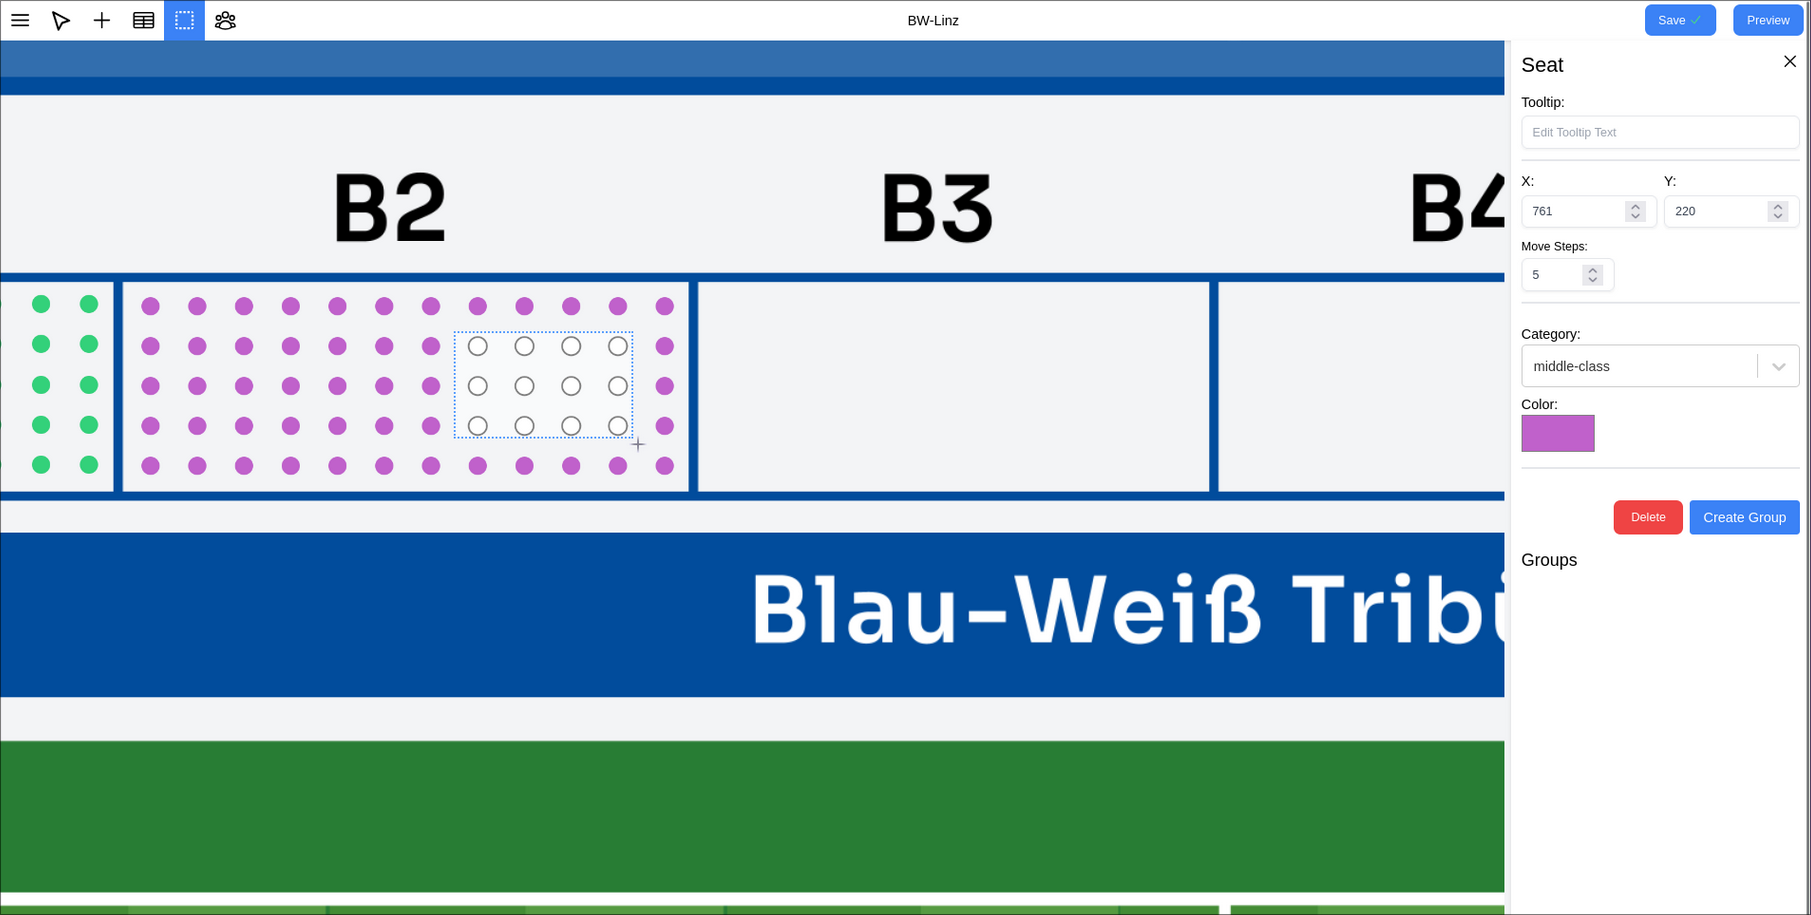
\includegraphics[scale=0.3]{pics/multiselect.png}
    \caption{Multiselect Tool}
    \label{fig:multiselect-tool}
\end{figure}

\begin{lstlisting}[language=Typescript, caption={Multiselect Tool},label={lst:multiselect-tool}]
    L.Map.Multiselect = L.Map.BoxZoom.extend({
        _onMouseMove: function (e) {
            var startPoint = _startPoint,
                box = this._box,

                layerPoint = this._map.mouseEventToLayerPoint(e),
                offset = layerPoint.subtract(startPoint),

                newPos = new L.Point(
                    Math.min(layerPoint.x, startPoint.x),
                    Math.min(layerPoint.y, startPoint.y));

            L.DomUtil.setPosition(box, newPos);

            box.style.width = (Math.max(0, Math.abs(offset.x) - 4)) + 'px';
            box.style.height = (Math.max(0, Math.abs(offset.y) - 4)) + 'px';
        },

        _onMouseUp: function (e) {
            this._finish();
            const map = this._map,
                layerPoint = map.mouseEventToLayerPoint(e);
            const bounds = new L.LatLngBounds(
                map.layerPointToLatLng(layerPoint),
                map.layerPointToLatLng(_startPoint)
            )

            if (_currFunction != null) {
                _currFunction(bounds);
            }
            _currFunction = null
        },
    })
\end{lstlisting}

The code uses parts of the original code concepts, and adapts them for the selection of seats. The original source can be found in Leaflet's source code.

This box is utilized not only for the multiselect tool, but also for the grid tool which is explained in more detail in section \ref{sec:grid-tool}. The modified functionality just disables the zoom of the original feature, and accepts a function that is called \texttt{onMouseUp} with the boundaries of the drawn rectangle as parameters. When the rectangle select is needed, it can be dynamically loaded into the map component.

Except for this tool, another way of selecting multiple seats at once was implemented, because of usability reasons and user expectations. In editors such as Photoshop, Gimp, and File Explorers, holding the \texttt{Ctrl} or \texttt{cmd} key while clicking on an object allows the user to select multiple objects. This was also implemented in SeatGen. The user can hold this key and click on a seat to select more than one seat.